\documentclass{article}
\usepackage{graphicx} % Required for inserting images
\usepackage{multirow}
\title{Tarea Automorfismo basado en redes neuronales}
\author{Esteban Rodriguez Muñoz }
\date{February 2023}
\graphicspath{ {./images/} }

\begin{document}

\maketitle

\section{¿Qué es una Autobahn y para qué sirve?}
Son un grupo de redes neuronales de grafos inspiradas en automorfismos. Funciona aplicando convoluciones en cada neurona en vez de nodos, estas son equivariantes(al aplicar una funcion de transformación de simetría y luego calcular la función produce el mismo resultado que calcular la función y luego aplicar la transformación) al grupo de automorfismo mantieniendo la forma de simetria de la permutacion global.

\section{ ¿Por qué los autores proponen utilizar los automorfismos de grafos para reflejar las simetrías internas de un grafo?}
Es de gran interes el desarrollo de grafos basados en redes neuronales para recolectar la informacion relacional pero para que esta sea confiable se requiere que mantengan la misma estructura inicial luego de trabajar con ellos.Otros metodos como redes neuronales que pasan mensajes han servido respetando la simetria del grafo luego de la permutacion de los nodos, estos no pueden distinguir grafos mas complejos y sus subestructuras.

El Autobahn tiene como objetivo crear redes neuronales flexibles y eficientes usando las simetrias de las subestructuras automorfas del grafo. El autobahn asocia las neuronas con subgrafos en vez de nodos o aristas para construir redes practicas de convoluciones.



\section{Pruebe los isomorfismos sugeridos por la (Figura 2.1 panel a)}


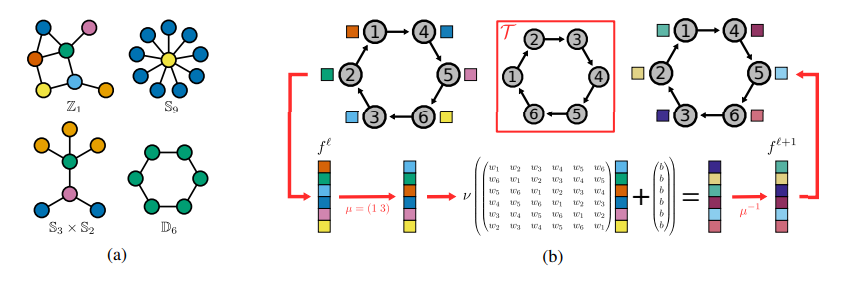
\includegraphics[scale=0.7]{grafos}




 
\begin{equation}
Edges Z1:{(az , ve),(az , na),(ro , ve),(na , ve),(ce , ve),(am , ce),(am , na),(ca , ce)}
\end{equation}
En los grafos mostrados en la figura (a), los nodos que estan en la misma orbita tienen el mismo color, siendo el primer grafo en el grupo Z1, todos tienen orbitas diferentes y no se pueden hacer permutaciones que no afecten el la simetria del grafo, ppr lo que su grupo de automorfismos estaria definido en el identidad y en la aplicacion de n \rightarrow -n. Asi que: Aut(Z) \cong c2


En el grafo descrito por S3xS2 podemos observar que los nodos "hoja" como llamariamos en una estructura de tipo arbol tienen la misma orbita en la parte superior e inferior (s3 y s2 respectivamente) La cantidad de posibles combinaciones estaria determinada por 3!*2! dandonos asi una tabla de combinaciones de automorfos los cuales pueden cambiar de posicion entre ellos sin cambiar la estructura original.

En el grafo descrito por S9, podemos observar que tiene 9 parejas de nodos, todas incluyen el nodo central, se pueden generar intercambios entre pares de nodos y dejando uno invariable, tambien la reflexion y rotacion de los nodos mantiene la estructura original que cumplen el automorfismo.

En el grafo D6 estudiado en clase, pudimos observar que girar 60 grados generan 6 nuevas posibles combinaciones, el usar su espejo y girar 60 grados nos darian 6 nuevas opciones, en una tabla de cayley de 12x12 podemos ver las posibles combinaciones de las convoluciones generadas.





\section{Explique en que consiste la Figura 2.1 panel b. ¿Cuál es su relación con el grupo de automorfismos de D_6?}

La figura del panel b seria una representacion de un grafo dirigido de 6 nodos, de forma ciclica en el cual se recorre el por todos sus vertices una sola vez, muestra como se hizo una permutacion entre el nodo (1,3), a su tabla de cayley podemos usar una operacion de suma para generar un nuevo grafo, al sacar la inversa de este nuevo grafo recuperariamos la forma del primer grafo. Un grafo dirigido como el del ejemplo B es una buena representacion del comportamiento del comportamiento de una permutacion ciclica con la cual podemos obtener grupos de simetrias del grupo diedral del D6 de forma de hexagono regular.



\end{document}

